\par Robots in general can be categorized into serial and parallel types. Serial robots are characterized by a series of linked joints while parallel robots have multiple axes that move in parallel, usually working together to support a single platform.

\par Parallel robots represent a significant branch in the field of robotics due to their precision and versatility in various applications such as pick-and-place manipulation, simulators, manufacturing, and tooling, among others. As described in \cite{shao2024}, these applications span both industry and medicine, leveraging the high rigidity, precision, and speed of these robots to compensate for the performance limitations of serial robots.

\par The origin of parallel robots dates back to the 1960s with the development of the Gough-Stewart \cite{stewart1965} parallel mechanism (Figure \ref{fig:stewart_platform}), which has become one of the most iconic in the field of parallel robotics. Later, in the 1980s, Reymond Clavel designed a robust parallel structure with three translational degrees of freedom and one rotational degree of freedom, as illustrated in Figure \ref{fig:delta_robot}. This robot, known as the Delta Robot, has become one of the most significant examples in the field of parallel robotics. 

% https://www.weiss-world.com/Productpics/handling/Pick%20%26%20Place/DR/dr.png
% https://actu.epfl.ch/news/the-delta-robot-swiss-made-and-fastest-in-the-worl/
% {stewart1965}
\begin{figure}
    \centering
    \begin{subfigure}[t]{0.45\textwidth}
        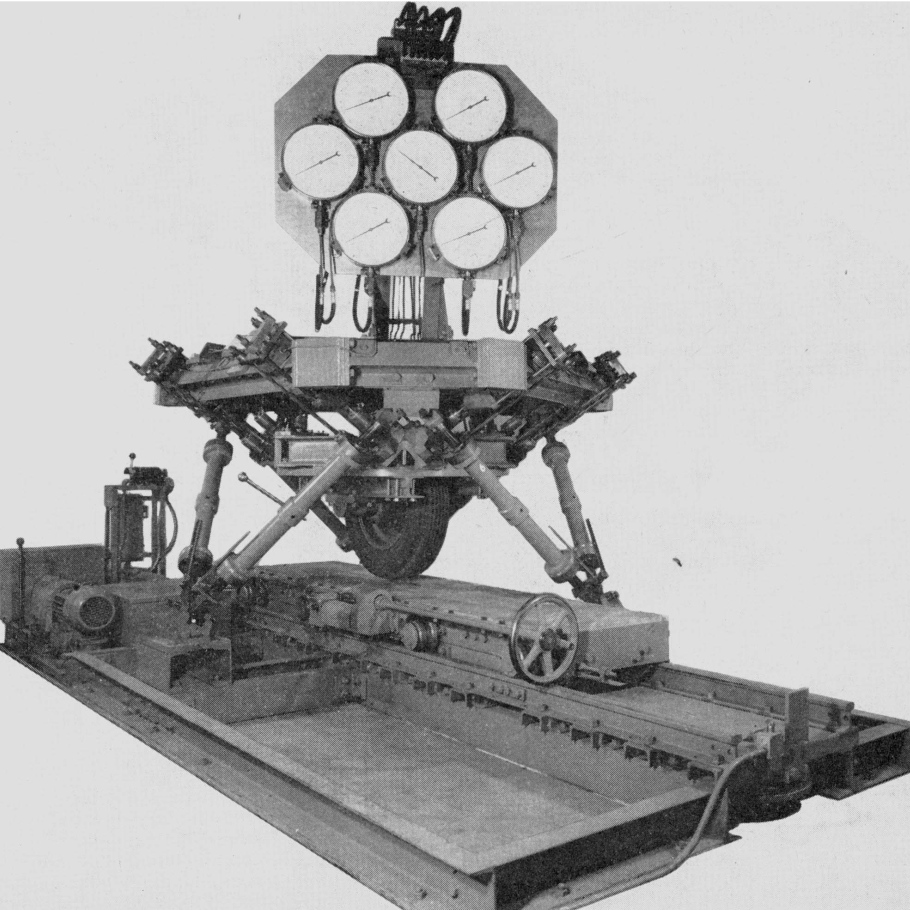
\includegraphics[width=\textwidth]{stewart_platform}
        \caption{Gough-Stewart Platform}
        \caption*{Source: Adapted from \cite{stewart1965}}
        \label{fig:stewart_platform}
    \end{subfigure}
    \begin{subfigure}[t]{0.45\textwidth}
        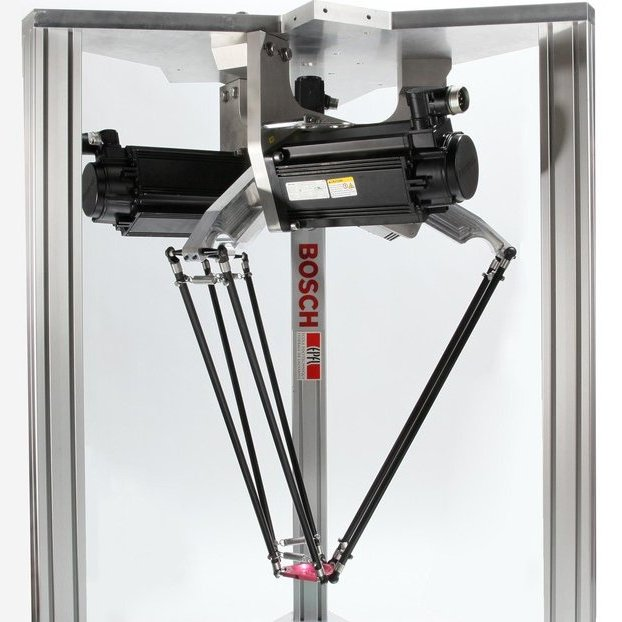
\includegraphics[width=\textwidth]{clavel_robot}
        \caption{Clavel's Delta Robot}
        \caption*{Source: Adapted from \cite{sandyEFPL}}
        \label{fig:delta_robot}
    \end{subfigure}
    \caption{Traditional parallel robots}
    \label{fig:traditionals}
\end{figure}

\par Another distinguishing feature of these robots is the presence of multiple closed kinematic chains that connect and move the mobile platforms, in contrast to serial robots, which operate with an open kinematic chain and move in a linear sequence. However, according to Briot and Kahrs\cite{briot2023} the fundamental questions about this class of robots have been addressed. As a result, in recent years, interest in parallel robots has shifted towards exploring new alternatives.

\par Current research in robotics transcends conventional definitions, pushing the boundaries of this field and fostering new possibilities and innovations. Briot and Kahrs \cite{briot2023} illustrate how parallel manipulators have been integrated into various novel robot types, such as continuum robots, flying robots, cable-driven robots, underactuated robots, multi-fingered hands, and micro-scale parallel robots. However, this emerging class of robots presents significant scientific challenges in design, modeling, and control. Among these categories, aerial robots, parallel robots, and continuum or soft robots are particularly noteworthy for their ability to venture into new areas due to their lightness and flexibility.

\par Expanding on these insights, Russo et al. \cite{russo2023} offer a comprehensive review focusing on recent advancements, current limitations, and ongoing challenges in the design, modeling, and control of continuum robots. They classify continuum robots based on their design, distinguishing them by their extrinsic or intrinsic actuation methods. Extrinsic actuation (Figure \ref{fig:extrinsic_continuum_robots}) involves transmitting motion from the robot's base along its structure, categorized into three main families depending on the transmission elements used: tendon-driven, concentric tube (Figures \ref{fig:concentric_tube}, \ref{fig:concentric_tube_ex}), and rod-driven robots (Figures \ref{fig:rod_driven}, \ref{fig:rod_driven_ex}). Furthermore, robots with intrinsic actuation employ actuators integrated into their structure to generate movement, meaning the actuation occurs within the robot's body.

\begin{figure}
    \centering
    \begin{subfigure}[b]{0.4\textwidth}
        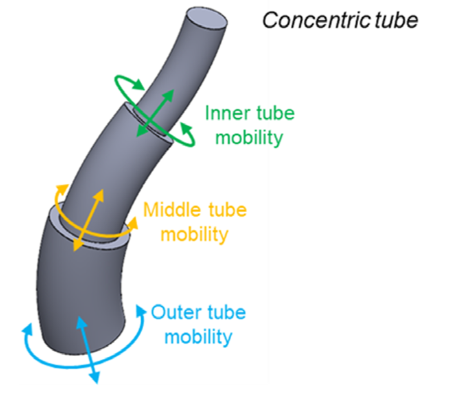
\includegraphics[width=\textwidth]{concentric_tube}
        \caption{Concentric tube robot mobility}
        \label{fig:concentric_tube}
    \end{subfigure}
    \begin{subfigure}[b]{0.4\textwidth}
        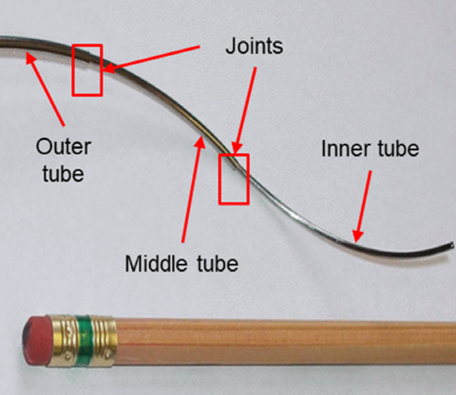
\includegraphics[width=\textwidth]{concentric_tube_example}
        \caption{Concentric tube prototype}
        \label{fig:concentric_tube_ex}
    \end{subfigure}
    \vskip\baselineskip
    \begin{subfigure}[b]{0.4\textwidth}
        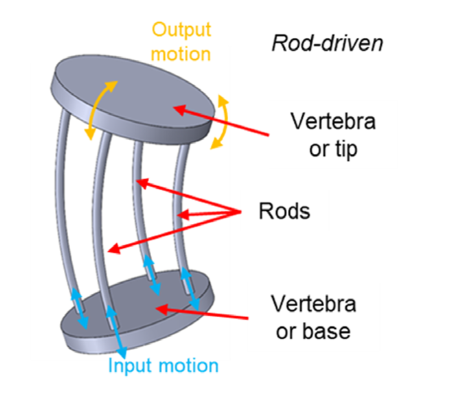
\includegraphics[width=\textwidth]{rod_driven}
        \caption{Rod-driven continuum robot conceptual scheme}
        \label{fig:rod_driven}
    \end{subfigure}
    \begin{subfigure}[b]{0.4\textwidth}
        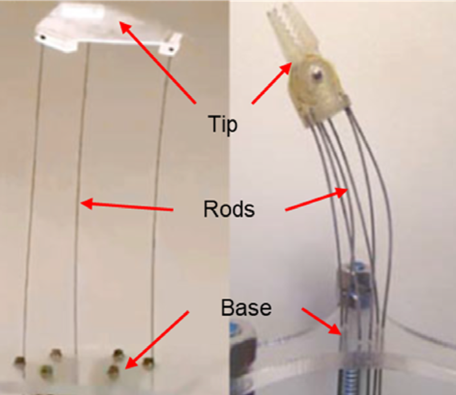
\includegraphics[width=\textwidth]{rod_driven_example}
        \caption{Parallel continuum rod-driven robot prototype}
        \label{fig:rod_driven_ex}
    \end{subfigure}
    \caption{Continuum robots with extrinsic actuation}
    \caption*{Adapted from }
    \label{fig:extrinsic_continuum_robots}
\end{figure}



\par Current challenges in designing and modeling parallel continuum robots include improving performance through miniaturization of actuators, integrating with rigid robots, exploring smart materials, precise environmental modeling, and implementing proprioception with new sensors \cite{russo2023}. Modeling efforts also focus on representing interaction environments and improving real-time implementations, alongside standardizing simulation environments. Control challenges involve ensuring precise manipulation and adapting to dynamic environments using advanced sensor technology and adaptive strategies

\par This project aims to address the efficiency challenges of continuum robots through the miniaturization of their parallel linear actuators. Specifically, it focuses on implementing adaptive control strategies for diverse applications using an extrinsic actuation platform for rod-driven continuum robots. This research endeavors to enhance affordability and user-friendliness, aiming to broaden adoption and usability in practical contexts.


\section{Objectives}

\subsection{General Objective}
To design and develop a portable, modular, and scalable platform with a control system for the actuation of rod-driven continuum parallel robots.

\subsection{Specific Objectives}
\begin{itemize}
    \item Adapt an existing design of a rod-driven continuum parallel robot, optimizing it for reduced size while maintaining functionality and performance.
    \item Design linear actuators that provide precise control and enable dexterous movements, ensuring high accuracy and reliability.
    \item Fabricate all necessary components and assemble a fully functional physical prototype of the platform, adhering to the design specifications.
    \item Implement a customized language specification for programming the linear actuators, allowing for tailored control and flexibility in operations.
    \item Develop an application to interface with the control system, utilizing the created protocol to facilitate seamless communication and control.
    \item Conduct comprehensive experimental testing and validation of the system, ensuring it meets all performance criteria and operational standards.
\end{itemize}